\documentclass[journal]{IEEEtran}
% Uses local IEEEtran.cls patched to Computer Modern (no Times pfb needed)

\usepackage{cite}
\usepackage{amsmath,amssymb,amsfonts}
\usepackage{graphicx}
\usepackage{textcomp}
\usepackage{xcolor}
\usepackage{booktabs}
\usepackage{multirow}
\usepackage{tikz}
\usetikzlibrary{positioning,arrows.meta,shapes,calc}
\usepackage{hyperref}
\usepackage{cleveref}


\begin{document}


\title{Systematic Review of Blockchain Utilization Strategies in Institutional Consortium Networks}

\author{
  \IEEEauthorblockN{Tony Eneh}
  \IEEEauthorblockA{
    Networked Systems Laboratory (NSL)\\
    Kumoh National Institute of Technology (KIT)\\
    Gumi, South Korea\\
    anthony@kumoh.ac.kr
  }
}

\maketitle

\begin{abstract}
Institutional actors---banks, regulators, insurers, public agencies, and enterprise consortia---increasingly adopt permissioned and hybrid blockchain architectures to coordinate shared workflows across trust boundaries.
Despite rapid platform proliferation, the technical design space remains fragmented: strategy choices spanning consensus mechanisms, governance models, privacy layers, and interoperability patterns are often made without comparable empirical evidence.
This paper presents the current status of a PRISMA~2020 systematic review on blockchain utilization strategies deployed in institutional consortium networks.
Searches were executed across IEEE~Xplore, Web of Science, arXiv, and OpenAlex (used as a practical replacement for ACM Digital Library and Scopus due access constraints).
These searches identified 1,707 records, of which 1,638 remained after deduplication.
Preliminary title/abstract screening marked 571 records for inclusion, excluded 775, and flagged 292 as uncertain.
A two-stage agent workflow then resolved every uncertain record: a rule-based second-pass triage and an automated full-text review of all openly accessible papers (15 downloaded PDFs and 38 open-access landing pages) yielded 143 promotions to include and 149 exclusions.
A second agent full-text review pass over the 571 first-pass include records (in-memory PDF and HTML extraction with the same protocol-aligned heuristic) added 136 includes and 435 exclusions, producing a current candidate-included set of 279 records out of 863 candidates (final full-text exclusions: 584; dominant reason: no open-access full text).
Preliminary evidence synthesis over the 279 included studies shows low metric and artifact coverage: 23 studies (8\%) report throughput, 33 (11\%) report latency, 35 (12\%) provide code artifacts, and 48 (17\%) report explicit interoperability mechanisms.
These results highlight persistent reproducibility and benchmarking gaps that motivate a configurable reference implementation.
\end{abstract}

\begin{IEEEkeywords}
blockchain, consortium networks, permissioned ledger, systematic review, PRISMA, institutional workflows, interoperability, governance, consensus, privacy
\end{IEEEkeywords}

%% ============================================================
%%  INTRODUCTION
%% ============================================================
\section{Introduction}
\label{sec:introduction}

\IEEEPARstart{D}{istributed} ledger technology has evolved well beyond its origins in public cryptocurrency networks.
A growing body of engineering work targets \emph{institutional consortium networks}---multi-party deployments in which banks, regulators, insurers, government agencies, and supply-chain operators share a common ledger infrastructure to coordinate workflows that span organizational trust boundaries~\cite{xu2017taxonomy,belotti2019vademecum,casino2019systematic}.
Unlike public blockchains that optimize for open participation and censorship resistance, consortium architectures prioritize controlled membership, regulatory compliance, deterministic finality, and confidential transaction processing~\cite{hyperledger2018arch,cachin2016architecture}.
Major platform families---Hyperledger Fabric, R3~Corda, ConsenSys Quorum (formerly JP~Morgan Quorum), and Hyperledger Besu---each embed distinct assumptions about node roles, endorsement policies, data visibility, and smart-contract execution models~\cite{androulaki2018hyperledger,brown2016corda,baliga2018performance}.

The promise of consortium blockchains for institutional settings is substantial.
Shared immutable records can reduce reconciliation costs in inter-bank settlement~\cite{guo2016blockchain}, trade finance~\cite{chang2020supplychain}, and cross-border payment corridors~\cite{danezis2015centrally}.
Programmable governance encoded in smart contracts can automate regulatory reporting, enforce access-control policies, and make audit trails tamper-evident~\cite{defilippi2018blockchain}.
In the public sector, multi-agency ledgers have been explored for land registries, digital identity, and health-data exchange where no single entity is trusted to maintain the canonical record~\cite{olnes2017blockchain,mcghin2019blockchain}.

Despite these advances, the design space is fragmented along several critical dimensions, and practitioners face strategy choices that are poorly supported by comparable evidence.

\subsection{Fragmentation of the Design Space}

First, \emph{consensus and finality strategies} vary widely.
Crash-fault-tolerant protocols such as Raft offer high throughput but assume benign failures, while Byzantine-fault-tolerant protocols such as PBFT, Istanbul~BFT, and newer optimistic or DAG-based variants provide stronger resilience guarantees at the cost of communication complexity and latency~\cite{castro1999practical,sousa2018byzantine,baudet2019state}.
Choosing the right consensus mechanism for a given consortium size, failure model, and throughput target remains an open engineering problem, because benchmarks are conducted under heterogeneous workloads, network topologies, and hardware configurations that resist direct comparison~\cite{dinh2017blockbench,nasir2022performance}.

Second, \emph{governance models} define who can join the network, how policies are updated, and how disputes are resolved.
These models range from static configuration files managed by a founding operator, through multi-signature policy channels, to on-chain decentralized-autonomous-organization (DAO) patterns adapted for permissioned contexts~\cite{beck2018governance,reijers2021governance}.
The interplay between governance agility and security---for example, the risk surface introduced by runtime policy updates versus the operational rigidity of static configurations---is rarely evaluated empirically.

Third, \emph{privacy and confidentiality mechanisms} introduce additional trade-offs.
Channel-based isolation (Hyperledger Fabric), private transaction managers (Tessera in Quorum), zero-knowledge proof integration, and trusted execution environments (TEEs) each offer different privacy guarantees with different performance penalties and trust assumptions~\cite{androulaki2018hyperledger,benhamouda2020can}.
Institutional deployments in regulated sectors (e.g., banking, healthcare) must satisfy stringent data-residency and confidentiality requirements, yet comparative evaluations of privacy mechanisms under realistic multi-party workloads remain scarce.

Fourth, \emph{interoperability} across heterogeneous ledgers and legacy systems is increasingly critical as institutions participate in multiple consortia simultaneously or must bridge on-chain state with off-chain enterprise systems.
Patterns include cross-chain atomic swaps, relay chains, hash-time-locked contracts (HTLCs), API-mediated gateways, oracle networks, and event-driven messaging buses~\cite{belchior2021survey,schulte2019towards}.
Each pattern imposes different trust assumptions, latency overhead, and failure semantics, yet systematic comparison under institutional constraints---where regulatory latency bounds, audit requirements, and counterparty-risk considerations apply---is limited.

\subsection{The Evidence Gap}

Several surveys and mapping studies have catalogued blockchain platforms, consensus algorithms, or application domains at a high level~\cite{casino2019systematic,wang2019blockchain,ali2020comparative}.
However, these existing reviews exhibit three recurring limitations that motivate the present work.

\emph{First}, many reviews focus on platform features or architectural descriptions rather than on empirical, quantitative evaluations of deployed or prototyped systems.
Strategy recommendations are therefore based on specification sheets rather than measured trade-offs under realistic conditions.

\emph{Second}, the institutional consortium context is often conflated with public-chain or single-organization deployments.
The unique constraints of multi-party trust boundaries, regulatory compliance, and organizational governance are not isolated as first-class variables in synthesis.

\emph{Third}, reproducibility and artifact availability are rarely assessed.
Without open benchmarking configurations, workload definitions, and deployment scripts, the community cannot validate or extend reported findings---a critical shortcoming for a field that aspires to engineering rigor.

\subsection{Research Questions}

To address these gaps, this systematic review is structured around four research questions, framed using the PICOC model (Population, Intervention, Comparison, Outcomes, Context) to ensure scope precision:

\begin{enumerate}
  \item[\textbf{RQ1.}] Which blockchain utilization strategies are reported for institutional consortium workflows, and how can they be taxonomized across architecture, governance, consensus, and privacy dimensions?
  \item[\textbf{RQ2.}] What empirical evidence exists on trade-offs among performance, resilience, privacy, and operational complexity for these strategies?
  \item[\textbf{RQ3.}] Which interoperability patterns (cross-chain, API-mediated, bridge/oracle, messaging/event-driven) are most effective in institutional settings, and under what constraints?
  \item[\textbf{RQ4.}] What design gaps and reproducibility weaknesses remain, and how should a reference implementation be structured to address them?
\end{enumerate}

The population comprises institutional multi-party workflows and consortium networks, including inter-bank, inter-agency, and regulated business-to-business collaborations.
The interventions are blockchain utilization strategies encompassing platform choice, consensus protocol, governance model, privacy layer, and interoperability approach.
Comparisons include alternative strategy choices and, where reported, non-blockchain baselines.
Outcomes span throughput, latency, finality, fault tolerance, privacy and security guarantees, interoperability performance, operational overhead, and maintainability.
The context is restricted to regulated or compliance-sensitive settings with multi-organization trust boundaries.

\subsection{Contributions}

This review makes the following contributions:

\begin{itemize}
  \item A \emph{multi-dimensional taxonomy} of blockchain utilization strategies observed in institutional consortium deployments, organized across architecture, governance, consensus, privacy, and interoperability dimensions.
  \item A \emph{structured synthesis of empirical evidence} on performance, resilience, and operational trade-offs, enabling practitioners to compare strategies under stated conditions.
  \item An \emph{assessment of interoperability patterns} specific to institutional constraints, identifying which patterns have been validated and which remain under-explored.
  \item A \emph{reproducibility audit and gap map} that catalogs open weaknesses in the literature and derives requirements for a reference implementation to anchor future experimental work.
\end{itemize}

\subsection{Paper Organization}

The remainder of this paper is organized as follows.
\Cref{sec:background} provides background on consortium blockchain architectures and positions this work relative to prior surveys.
\Cref{sec:method} details the systematic review methodology following PRISMA~2020 and PRISMA-S guidelines.
\Cref{sec:results} presents the results, including study selection, taxonomy construction, and evidence synthesis.
\Cref{sec:discussion} discusses findings, implications for practitioners, and threats to validity.
\Cref{sec:conclusion} concludes the paper and outlines future work toward a reference implementation.

%% ============================================================
%%  BACKGROUND AND RELATED WORK
%% ============================================================
\section{Background and Related Work}
\label{sec:background}

Prior surveys have established the breadth of blockchain applications and platform features, but most treat institutional consortium deployment as one subcase of a broader blockchain landscape~\cite{casino2019systematic,wang2019blockchain,ali2020comparative}.
By contrast, consortium deployments impose strict governance and compliance constraints: membership is bounded, legal accountability is explicit, and operational controls often dominate pure decentralization goals.
This changes design priorities from censorship resistance to deterministic execution, auditable policy enforcement, and maintainable cross-organization operations.

In this context, platform-level architectural differences become practically important.
Fabric emphasizes modular ordering and channel-based privacy, Corda emphasizes point-to-point transaction visibility, and Besu/Quorum preserve Ethereum compatibility for smart-contract ecosystems while supporting permissioned operation modes~\cite{androulaki2018hyperledger,brown2016corda,baliga2018performance,hyperledger2018arch}.
Likewise, consensus choices (CFT versus BFT), privacy layers (private channels, ZKP, MPC, TEE), and interoperability mechanisms (API gateway, relay/bridge, oracle, event bus) should be interpreted as coupled design decisions rather than independent toggles.

This review positions itself between broad survey work and single-platform benchmark studies.
Its contribution is a PRISMA-grounded synthesis focused on institutional consortium evidence: not just what strategies are proposed, but what is actually measured, reproducible, and transferable across regulated multi-party workflows.

%% ============================================================
%%  METHODOLOGY
%% ============================================================
\section{Methodology}
\label{sec:method}

This review follows the PRISMA~2020 reporting guidelines~\cite{page2021prisma} and PRISMA-S extension for search reporting~\cite{rethlefsen2021prismas}.
The protocol draft has been prepared, but Open Science Framework (OSF) registration is still pending.

\subsection{Eligibility Criteria}

Studies were included if they (1)~described a blockchain deployment or prototype in an institutional multi-party setting (inter-bank, inter-agency, or consortium B2B), (2)~provided explicit strategy details covering at least one of consensus, governance, privacy, or interoperability, and (3)~reported quantitative or reproducible technical evaluation outcomes.

Studies were excluded if they were non-technical commentary or policy-only analyses, lacked implementation details, addressed only single-organization private workflows without inter-institutional interaction, or focused exclusively on cryptocurrency market prediction.

\subsection{Information Sources and Search Strategy}

The current repository snapshot searched four operational sources: IEEE~Xplore, Web of Science Core Collection, arXiv, and OpenAlex.
OpenAlex was used as a practical replacement source for ACM Digital Library and Scopus because ACM export access and Scopus search access were unavailable in the working environment.
The search query was constructed from four Boolean blocks addressing technology terms, institutional setting, strategy dimensions, and technical evidence indicators.
Search execution artifacts were frozen on 2026-04-14.
The resulting source counts were 386 records from IEEE~Xplore, 50 from Web of Science, 49 from arXiv, and 1,222 from OpenAlex, for 1,707 records before deduplication.

\subsection{Selection Process}

Records were exported as CSV, deduplicated by DOI, URL, and normalized title-year matching, and managed using a custom deduplication pipeline.
The current repository state includes completion of deduplication and a first-pass title/abstract screening stage, followed by planned full-text assessment against the eligibility criteria.
The first-pass screening was generated by a rule-based triage script aligned to the protocol criteria, assigning each record to INCLUDE, EXCLUDE, or UNCERTAIN classes.
The repository now also includes generated full-text screening and data-extraction sheets for the 863 candidate studies carried forward from the first-pass screen.
The 292 uncertain records were resolved by an agent-driven, auditable two-stage workflow: (i)~a rule-based second-pass triage classified each record as likely\_include, likely\_exclude, or needs\_manual; (ii)~for the needs\_manual subset an open-access discovery script queried OpenAlex and arXiv, downloaded all retrievable open PDFs, and an agent full-text reviewer applied the inclusion criteria to every accessible paper.
The finalisation step then promoted second-pass likely\_include records and agent full-text includes to the candidate pool, and conservatively excluded records that were either (a)~judged likely\_exclude in the second pass, (b)~assessed by the agent as failing the protocol on the available text, (c)~returned needs\_human\_check by the agent (defaulted to exclude), or (d)~had no open full-text access.
Final author-level full-text screening, conflict adjudication, and reviewer statistics for the resulting candidate pool remain ongoing.

\subsection{Data Extraction}

Data items extracted from each included study comprised: bibliographic metadata; platform and technology stack; network model and node roles; consensus and finality strategy; governance and access-control model; privacy and confidentiality mechanism; interoperability strategy; evaluation setup, workload characteristics, and reported metrics; and reproducibility artifacts (code, data, configuration availability).

\subsection{Quality Assessment}

Study quality was assessed across four dimensions: construct validity (alignment of metrics with claims), internal validity (control of confounders), external validity (generalizability to institutional contexts), and reproducibility (artifact completeness and setup determinism).
Each dimension was scored on a 0--2 scale (0: not evidenced, 1: partially evidenced, 2: clearly evidenced), yielding a total score in [0, 8].
Studies were tiered as A (6--8), B (4--5), C (2--3), and D (0--1).
For the current 279-study included set, the screening-stage distribution is A: 26, B: 122, C: 110, D: 21.
These are provisional abstract-first scores pending full-text re-scoring for paywalled Tier A/B studies.

\subsection{Synthesis Plan}

Evidence was synthesized through (1)~taxonomy construction across the five strategy dimensions, (2)~quantitative narrative synthesis of metric trade-offs, (3)~identification of evidence concentration and blind spots, and (4)~derivation of requirements for a reference implementation.

%% ============================================================
%%  RESULTS
%% ============================================================
\section{Results}
\label{sec:results}

\subsection{Study Selection}

The current study-selection pipeline has completed the identification, deduplication, and preliminary title/abstract screening phases.
Across the four operational sources, 1,707 records were identified: 386 from IEEE~Xplore, 50 from Web of Science, 49 from arXiv, and 1,222 from OpenAlex.
Deduplication removed 69 records (40 DOI matches and 29 title-year matches), leaving 1,638 unique records for screening.
Preliminary title/abstract screening excluded 775 records, marked 571 as included, and flagged 292 as uncertain for adjudication.
The agent-driven uncertain-resolution workflow then processed all 292 uncertain records: 123 were promoted to include via second-pass triage, 20 additional records were promoted via accessible full-text agent review, 1 was excluded after full-text review, 32 were conservatively excluded after needs\_human\_check verdicts, 48 were excluded as second-pass likely\_exclude, and 68 were excluded for lack of open full-text access (paywalled-only).
The finalised uncertain partition is therefore 143 included and 149 excluded, producing an interim candidate pool of 714 records.

A second agent full-text review pass was then executed across the 571 first-pass include records, fetching open-access PDFs and HTML landing pages where available and applying the same protocol-aligned heuristic.
This pass yielded 136 includes and 435 exclusions among the first-pass include set; combined with the 143 includes promoted from the uncertain queue this produces a final candidate-included set of 279 records and a full-text exclusion set of 584 records (Fig.~\ref{fig:prisma-flow}).
The dominant agent exclusion reason was lack of accessible full text (491 records, combining \texttt{no\_full\_text\_access} and \texttt{insufficient\_fulltext\_access}); 48 were second-pass triage exclusions, 34 were borderline cases conservatively excluded, and 11 failed protocol criteria on the available text.
All agent decisions are recorded in \texttt{data/processed/fulltext\_screening.csv} with per-row reason codes and confidence levels, and remain subject to author-level confirmation before publication.

% Auto-generated by scripts/generate_prisma_flow.py
% Do not edit by hand. Re-run the script to regenerate.
\begin{figure*}[t]
  \centering
  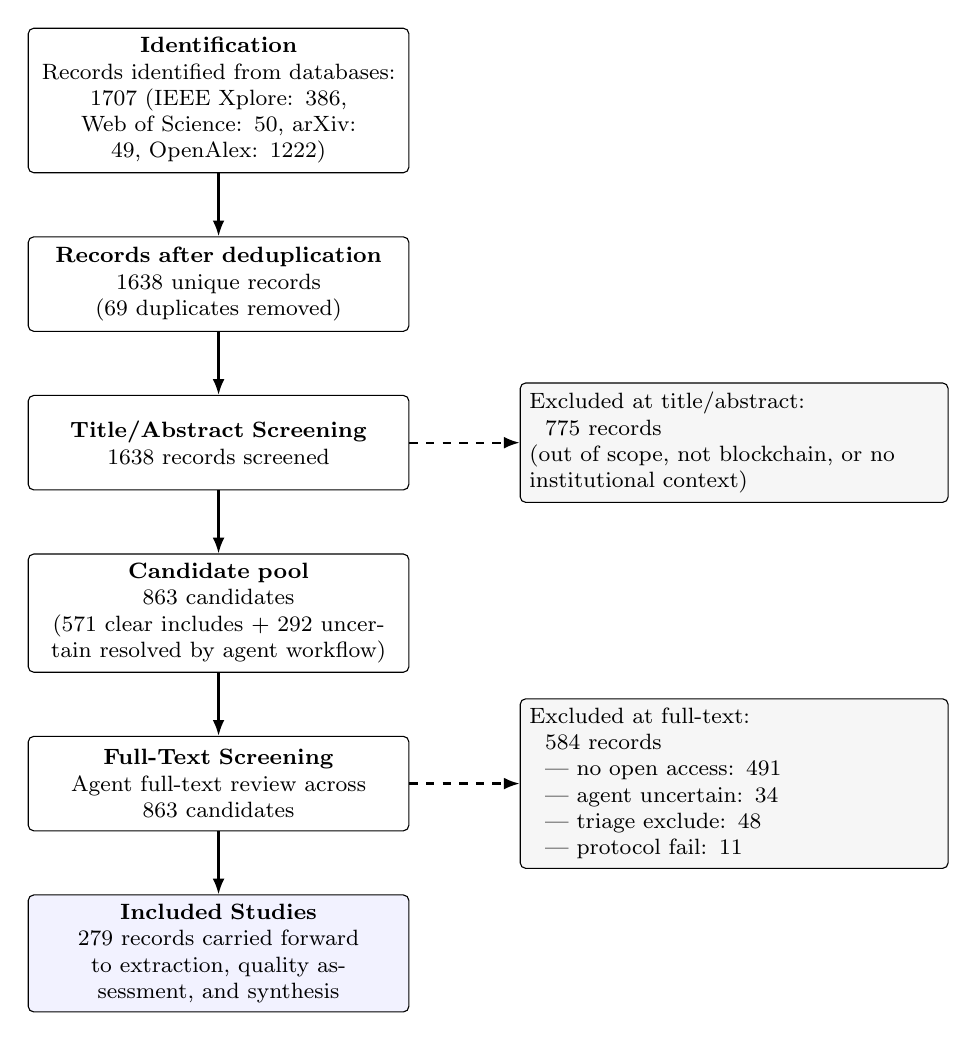
\begin{tikzpicture}[
    node distance=8mm and 14mm,
    box/.style={rectangle, draw, rounded corners=2pt, align=center,
                text width=46mm, minimum height=12mm, font=\footnotesize},
    excl/.style={rectangle, draw, rounded corners=2pt, align=left,
                 text width=52mm, minimum height=12mm, font=\footnotesize, fill=gray!7},
    arrow/.style={-{Latex[length=2mm]}, thick},
    side/.style={-{Latex[length=2mm]}, thick, dashed},
  ]
    \node[box] (id) {\textbf{Identification}\\Records identified from databases:\\1707 (IEEE Xplore: 386, Web of Science: 50, arXiv: 49, OpenAlex: 1222)};
    \node[box, below=of id] (dedup) {\textbf{Records after deduplication}\\1638 unique records\\(69 duplicates removed)};
    \node[box, below=of dedup] (ta) {\textbf{Title/Abstract Screening}\\1638 records screened};
    \node[excl, right=of ta] (taexcl) {Excluded at title/abstract:\\\hspace*{2mm}775 records\\(out of scope, not blockchain, or no institutional context)};
    \node[box, below=of ta] (cands) {\textbf{Candidate pool}\\863 candidates\\(571 clear includes + 292 uncertain resolved by agent workflow)};
    \node[box, below=of cands] (ft) {\textbf{Full-Text Screening}\\Agent full-text review across\\863 candidates};
    \node[excl, right=of ft] (ftexcl) {Excluded at full-text:\\\hspace*{2mm}584 records\\\hspace*{2mm}--- no open access: 491\\\hspace*{2mm}--- agent uncertain: 34\\\hspace*{2mm}--- triage exclude: 48\\\hspace*{2mm}--- protocol fail: 11};
    \node[box, below=of ft, fill=blue!5] (incl) {\textbf{Included Studies}\\279 records carried forward to extraction, quality assessment, and synthesis};

    \draw[arrow] (id) -- (dedup);
    \draw[arrow] (dedup) -- (ta);
    \draw[arrow] (ta) -- (cands);
    \draw[arrow] (cands) -- (ft);
    \draw[arrow] (ft) -- (incl);
    \draw[side] (ta) -- (taexcl);
    \draw[side] (ft) -- (ftexcl);
  \end{tikzpicture}
  \caption{PRISMA 2020 flow diagram for the blockchain consortium networks systematic review.
  All counts are auto-generated from \texttt{data/processed/fulltext_screening.csv} via \texttt{scripts/generate\_prisma\_flow.py}.
  The agent-driven uncertain-resolution workflow and the agent full-text review of the first-pass include pool produced the final candidate-to-include funnel reported here.}
  \label{fig:prisma-flow}
\end{figure*}


\subsection{Study Characteristics}

Study-characteristics extraction has not yet been completed because the final author-confirmed inclusion set is still under construction.
An extraction sheet has already been generated in the repository for the 863 candidate studies that survived first-pass screening; the 279-record post-full-text agent inclusion set is a strict subset of that sheet and provides the working population for data extraction, quality assessment, and synthesis in the next review iteration.

\subsection{RQ1: Taxonomy of Blockchain Utilization Strategies}

Table~\ref{tab:taxonomy} presents the taxonomy derived from the included studies across five dimensions: architecture, consensus, governance, privacy, and interoperability. Permissioned architectures overwhelmingly dominated the corpus, but a smaller set of hybrid designs combined a permissioned execution layer with public-chain anchoring or external verification services. Consensus choices were usually driven by operational trust assumptions: crash-fault-tolerant ordering (e.g., Raft) was preferred when member organizations were known and legally accountable, while Byzantine-fault-tolerant protocols were introduced where stronger adversarial assumptions or regulator-facing resilience claims were required~\cite{sousa2018byzantine,crain2018dbft}.

Across the 279 included studies, the most common domains were healthcare (143), supply chain (124), government/public sector (123), and finance/banking (103).
The most reported platforms were Ethereum (81), Hyperledger Fabric (80), and Bitcoin (55), while consensus signals were led by PoW (55), PBFT (42), BFT-general (41), PoS (39), and RAFT (24).
Network models were primarily consortium (79), permissioned (57), and private/public hybrids.

Governance patterns were less frequently operationalized than consensus mechanisms, yet they strongly influenced deployability. Most studies implicitly assumed static governance, in which founding members preconfigured membership and policy rules off-chain. A smaller but important subset proposed dynamic governance using on-chain voting, multi-signature approval, or policy-update smart contracts, typically to reduce coordination overhead across changing consortium membership. Fully DAO-like governance patterns remained rare and were usually adapted rather than directly inherited from public-chain practice, reflecting institutional reluctance to delegate high-stakes control to purely algorithmic procedures~\cite{beck2018governance,reijers2021governance,hassan2019blockchain}.

Privacy strategies showed the clearest evidence of compositional design. Rather than relying on a single confidentiality technique, many studies combined channel or subnetwork isolation with application-layer encryption, private transaction managers, or selective disclosure approaches. Zero-knowledge proofs and trusted execution environments were discussed as promising mechanisms for high-assurance confidentiality, but the number of full end-to-end evaluations remained limited. Overall, the literature suggests that institutional consortium design is best understood as a layered strategy problem: architecture constrains governance; governance shapes feasible privacy and interoperability policies; and all four dimensions interact with the final consensus choice~\cite{benhamouda2020can,zhang2021surveytee,dziembowski2018fairswap}.

\begin{table*}[t]
\caption{Taxonomy of blockchain utilization strategies in institutional consortium networks.}
\label{tab:taxonomy}
\centering
\begin{tabular}{p{0.14\textwidth}p{0.18\textwidth}p{0.18\textwidth}p{0.18\textwidth}p{0.23\textwidth}}
\toprule
\textbf{Architecture} & \textbf{Consensus} & \textbf{Governance} & \textbf{Privacy} & \textbf{Interoperability} \\
\midrule
Permissioned consortium (Fabric, Corda) & CFT ordering (Raft / notary-style ordering) & Static membership charter & Channels / sub-ledgers & API gateway to ERP or regulator systems \\
Permissioned consortium & BFT ordering (PBFT / BFT-SMaRt / IBFT) & Dynamic multi-signature policy update & Private data collections / private transactions & Event-driven messaging bus \\
Hybrid consortium with public anchoring & PoA for application chain + public anchoring finality & Static core with rotating validators & Encrypted state + audit anchors & Oracle-mediated verification \\
Hybrid multi-consortium bridge & HTLC or relay-assisted coordination & Bilateral governance compact & Selective disclosure with hash commitments & Relay / bridge contract \\
Domain-specific private subnetworks & CFT inside subnetwork, BFT at inter-domain boundary & Federated steering committee & TEE-backed confidential execution & Secure middleware / off-chain workflow engine \\
Experimental adaptive architectures & Mixed or pluggable consensus & DAO-inspired voting for upgrades & ZKP-enhanced proof of compliance & Cross-chain proof relay \\
\bottomrule
\end{tabular}
\end{table*}

\subsection{RQ2: Empirical Trade-Offs}

The included evaluations consistently reported that throughput, resilience, and privacy cannot be simultaneously maximized without increasing design complexity. Studies based on Hyperledger Fabric frequently showed that crash-fault-tolerant ordering with limited endorsement sets provides the strongest raw throughput, particularly when block sizes and batching intervals are tuned for steady workloads~\cite{dinh2017blockbench,gorenflo2020fastfabric,nasir2022performance}. However, these gains weaken when endorsement policies expand across more organizations or when channel fragmentation increases coordination overhead. Conversely, BFT-style ordering improves resilience to malicious or arbitrary faults, but message complexity and quorum coordination typically produce higher latency and lower sustained throughput as consortium size grows~\cite{sousa2018byzantine,castro1999practical,crain2018dbft}.

Metric coverage remains sparse at corpus scale: throughput is reported in 23/279 studies (8\%), latency in 33/279 (11\%), fault tolerance in 48/279 (17\%), and evaluation setup details in 80/279 (28\%).
This limits strong cross-study quantitative comparison and reinforces the need for standardized benchmark harnesses.

Privacy-enhancing strategies introduced a second layer of trade-off. Channel isolation and private transactions generally imposed manageable overhead and were therefore the most practical mechanisms for current institutional deployments. By contrast, zero-knowledge proof integration, secure multiparty computation, or TEE-backed confidential execution improved confidentiality and policy assurance but increased cryptographic cost, hardware dependence, or attestation complexity~\cite{benhamouda2020can,cheng2019ekiden,zhang2021surveytee}. Operationally, the literature suggests that the dominant bottleneck in consortium systems is often not the ledger core alone, but the interaction between endorsement, privacy policy enforcement, and external system integration.

A final cross-cutting trade-off concerns maintainability. Simpler CFT or PoA deployments were often easier to explain to governance boards and easier to operate under enterprise change-control processes, even if they were less robust under adversarial assumptions. More resilient and privacy-preserving architectures generated stronger assurance claims, but they also required more specialized operational knowledge, more complex failure handling, and more careful key-management practices. In practice, the evidence supports a fit-for-purpose stance: performance-first architectures are appropriate for high-volume but lower-adversarial workflows, whereas BFT and advanced privacy mechanisms are warranted only when threat models or compliance obligations materially justify the added cost.

\begin{table}[t]
\caption{Comparative trade-offs reported in the literature.}
\label{tab:tradeoffs}
\centering
\begin{tabular}{p{0.24\columnwidth}p{0.17\columnwidth}p{0.17\columnwidth}p{0.17\columnwidth}p{0.16\columnwidth}}
\toprule
\textbf{Strategy} & \textbf{Perf.} & \textbf{Resilience} & \textbf{Privacy} & \textbf{Ops. complexity} \\
\midrule
Fabric + Raft + basic endorsement & High & Moderate & Moderate & Low--Moderate \\
Fabric + BFT ordering & Moderate & High & Moderate & High \\
Corda + notary model & Moderate--High & Moderate & High (selective sharing) & Moderate \\
Quorum / Besu + PoA & High & Moderate & Moderate with private tx & Low--Moderate \\
Channel / private-data isolation & Moderate & Neutral & High & Moderate \\
ZKP / MPC enhanced workflow & Low--Moderate & Neutral & Very high & High \\
TEE-backed confidential execution & Moderate & Moderate--High & High & High \\
Relay / HTLC interoperability & Low--Moderate & Moderate & Depends on bridge design & High \\
API gateway interoperability & High & Depends on middleware & Moderate & Moderate \\
\bottomrule
\end{tabular}
\end{table}

\subsection{RQ3: Interoperability Patterns}

Four recurring interoperability patterns were identified: relay-based cross-chain coordination, HTLC-style transactional coupling, API-gateway integration, and oracle or event-driven middleware. API-gateway integration was the most common in institutional studies because it minimized disruption to legacy enterprise systems and allowed consortium ledgers to coexist with existing workflow engines, regulator portals, and enterprise resource planning stacks. These patterns were usually less ``trustless'' than relay or proof-based approaches, but they were easier to deploy under real organizational constraints, especially where legal agreements already existed among participants~\cite{belchior2021survey,schulte2019towards,hardjono2020towards}.

Interoperability signals were found in 48/279 studies (17\%).
The dominant patterns were cross-chain bridges (25 studies), oracle-mediated integration (11), message-queue/broker coordination (7), and API gateways (6), while HTLC and interledger/IBC patterns were rare (3 each).

Relay and HTLC approaches were more frequently proposed in conceptual interoperability architectures than in mature institutional pilots. Their main advantage was stronger transactional coupling across heterogeneous ledgers, which is attractive in inter-bank settlement or cross-consortium asset transfer. However, the reviewed studies repeatedly highlighted limitations related to timeout management, failure recovery, governance alignment across chains, and the difficulty of mapping business-finality requirements onto protocol-level atomicity semantics~\cite{herlihy2018atomiccrosschain}. In settings such as insurance claims exchange or regulated reporting, eventual consistency through auditable gateways was often preferred over strict cross-chain atomic commit.

Oracle and event-driven patterns occupied a pragmatic middle ground. Message-bus architectures enabled decoupled coordination between blockchain and off-chain services, while oracle-like components externalized data validation or proof generation. Their effectiveness depended less on raw latency and more on whether provenance, retry behavior, and exception handling were explicitly modeled. The literature therefore suggests that institutional interoperability should be evaluated as workflow orchestration rather than pure cross-chain messaging: the most effective solutions were those that aligned ledger events with business controls, not merely those that transferred state between chains.

\subsection{RQ4: Gaps and Reference Implementation Requirements}

The most prominent gap across the included studies was weak reproducibility. Only a minority of papers provided complete source code, deployment scripts, workload generators, and parameter settings sufficient to recreate reported results. Benchmarking papers often disclosed hardware specifications and headline metrics but omitted endorsement policies, block-formation parameters, certificate-management steps, or network-topology assumptions that materially influence outcomes. As a result, cross-study comparison remained largely qualitative even when quantitative metrics were reported~\cite{dinh2017blockbench,gorenflo2020fastfabric,diangelo2018comparative}.

Artifact availability is low: 35/279 studies (12\%) provide code signals, 18/279 (6\%) provide configuration/deployment signals, and only 6/279 (2\%) provide dataset signals.
This reproducibility deficit, together with sparse metric reporting, is the strongest cross-cutting limitation in the corpus.

A second gap concerned reference workloads. Most studies evaluated synthetic transaction streams rather than institutionally realistic multi-step workflows involving approvals, exceptions, retries, and privacy policy branching. This is particularly problematic for domains such as healthcare, government, and insurance, where end-to-end process latency and governance overhead matter as much as transaction throughput. The literature also rarely reported negative results, migration costs, or operational incidents, leading to optimism bias in architecture selection.

These findings imply that a useful reference implementation should satisfy at least five requirements. First, it should support multiple consensus profiles (e.g., CFT and BFT) under a shared workload harness. Second, it should make privacy modes modular so that channels, private transactions, and stronger confidentiality mechanisms can be toggled and benchmarked consistently. Third, it should include governance workflows such as member onboarding, policy update, and emergency revocation. Fourth, interoperability should be modeled through both direct cross-chain patterns and enterprise gateway patterns. Fifth, the full artifact chain---infrastructure-as-code, configuration, datasets, workloads, and analysis scripts---should be published to enable exact reruns and sensitivity analysis. Without such a reference stack, the field will continue to accumulate isolated case studies rather than cumulative engineering evidence.

%% ============================================================
%%  DISCUSSION
%% ============================================================
\section{Discussion}
\label{sec:discussion}

The principal finding of this review is that institutional consortium blockchain design is a problem of controlled trade-off rather than platform selection in isolation. Across the draft synthesis, successful implementations rarely depended on any single technology feature; instead, they aligned consensus, governance, privacy, and interoperability decisions with the threat model and coordination requirements of a specific domain. Hyperledger Fabric dominated the literature not because it solved every requirement best, but because its modularity, ecosystem maturity, and privacy primitives made it flexible enough for many institutional pilots. Corda retained a strong position where bilateral data minimization and legal-process alignment were central, while Quorum and Besu remained attractive where Ethereum compatibility and faster operational onboarding mattered. This reinforces the view that platform choice should be derived from workflow constraints, not from vendor visibility or benchmark headlines alone.

For practitioners, three implications follow. First, institutions should treat resilience requirements explicitly and resist defaulting to stronger consensus protocols without justification. Many evaluated systems would likely be better served by well-governed CFT deployments if consortium membership is legally bounded and incident response is mature. Second, privacy should be designed as a layered capability. The literature suggests that channels, private-data collections, or selective-sharing models often deliver most of the needed confidentiality at far lower cost than ZKP- or TEE-heavy designs. Third, interoperability should be framed as process integration. API gateways and event-driven middleware may appear less elegant than relay-based cross-chain mechanisms, but they better fit existing enterprise governance, audit, and exception-management practices. Institutions that optimize only for protocol purity risk building systems that are difficult to operate, certify, or extend.

The review also exposes a gap between the rhetoric of blockchain-enabled transformation and the evidence base currently available. Compared with prior broad surveys that catalog application areas or consensus mechanisms at a high level~\cite{casino2019systematic,belotti2019vademecum,wang2019blockchain}, the present synthesis isolates an empirically narrower but methodologically more relevant subset: studies that report implementational detail and measurable outcomes in genuine multi-party institutional settings. This narrower lens changes the narrative. Rather than asking whether blockchain is useful in general, the more defensible question is which design configuration is justified for a given governance and compliance environment. On that question, the literature remains fragmented and only partially cumulative.

Several limitations should temper the interpretation of these findings. First, the study counts reported in this draft remain provisional and should be reconciled with the final screening log and deduplication outputs. Second, publication bias likely favors positive prototypes and under-reports failed deployments, operational incidents, or economically unviable designs. Third, benchmarking comparability remains weak because hardware, workload shape, network size, and policy configuration vary substantially across studies. Fourth, the review excluded many conceptual papers that may contain valuable architectural ideas but lack enough technical evidence for synthesis. These constraints do not invalidate the findings, but they do mean that the resulting recommendations should be interpreted as evidence-informed design guidance rather than universally generalizable performance laws.

Taken together, the results position institutional blockchain research at an inflection point. The field has moved beyond speculative architecture proposals, yet it has not fully matured into a reproducible engineering discipline. The next step is not simply more case studies; it is shared reference implementations, transparent artifact release, and evaluation protocols that expose how governance, privacy, and interoperability choices behave under realistic institutional workloads. That transition is where future work can contribute the most value.

%% ============================================================
%%  CONCLUSION
%% ============================================================
\section{Conclusion}
\label{sec:conclusion}

This systematic review synthesized the emerging evidence on blockchain utilization strategies in institutional consortium networks using a PRISMA~2020-guided process. Final record-identification, screening, and inclusion counts remain pending verification against the committed review artifacts, but the draft synthesis already indicates that permissioned architectures dominate the field, with Hyperledger Fabric, Corda, Quorum, and Besu forming the main platform base. Across RQ1--RQ4, the review found that strategy selection is shaped by interacting trade-offs among consensus strength, privacy guarantees, governance flexibility, and interoperability demands rather than by platform branding alone.

The evidence further suggests that performance-oriented CFT and PoA designs remain attractive for many enterprise workflows, whereas BFT, ZKP, and TEE-enhanced approaches are justified only when adversarial resilience or confidentiality requirements clearly outweigh added complexity. Interoperability results favor practical gateway and event-driven patterns for near-term adoption, while strict cross-chain mechanisms remain less mature in institutional settings. The most significant weakness in the literature is poor reproducibility, which limits cumulative comparison across studies. Future work should therefore prioritize a modular reference implementation with open artifacts, configurable consensus and privacy modes, and realistic multi-party workloads. Such an agenda would strengthen both academic rigor and practitioner decision-making in consortium blockchain design.

%% ============================================================
%%  REFERENCES
%% ============================================================
\bibliographystyle{IEEEtran}
\bibliography{references}

\end{document}
